\documentclass[hidelinks,12pt]{article}
\usepackage[a4paper,width=150mm,top=25mm,bottom=25mm]{geometry}
\usepackage[utf8]{inputenc}
\usepackage{graphicx}
\usepackage{amsmath}
\usepackage{amssymb}
\usepackage{apacite}
\usepackage{natbib}
\usepackage{hyperref}
\usepackage{float}
\usepackage{ragged2e}
\usepackage[font={footnotesize,bf}]{caption}
\usepackage[nottoc,numbib]{tocbibind}
\usepackage{multirow}
\usepackage{placeins}
\usepackage{booktabs}
\usepackage{hyperref}
\hypersetup{
    colorlinks=true,
    linkcolor=blue,
    filecolor=magenta,      
    urlcolor=cyan,
    pdftitle={Overleaf Example},
    pdfpagemode=FullScreen,
    }


\linespread{1.5}

\begin{document}

\begin{titlepage}
    \begin{center}
        \vspace*{1cm}
        
        
        % \vfill
        
        \large
        \textbf{Big Data Asset Pricing \\ Exercise 3: Factor Replication Analysis}
            
        
        \normalsize
        Seyyed Morteza Aghajanzadeh \\
        Department of Finance \\
        Stockholm School of Economics
        
        \vfill
        \normalsize
        \justifying
        \noindent
        \textbf{Statement:} I certify with my signature that I have solved the exercise according to the Code of Professional Conduct and Ethics. 
        For example, I have not plagiarized others, but, instead, solved the exercise myself (possibly with allowed collaboration with other students), and I have referenced my sources appropriately.

        \vfill
        
        \vspace{0.8cm}
            
        
        \vspace{0.8cm}
        \normalsize
        \centering
        2024-01
            
    \end{center}
\end{titlepage}

\section{}

\begin{figure}[htbp]
    \centering
    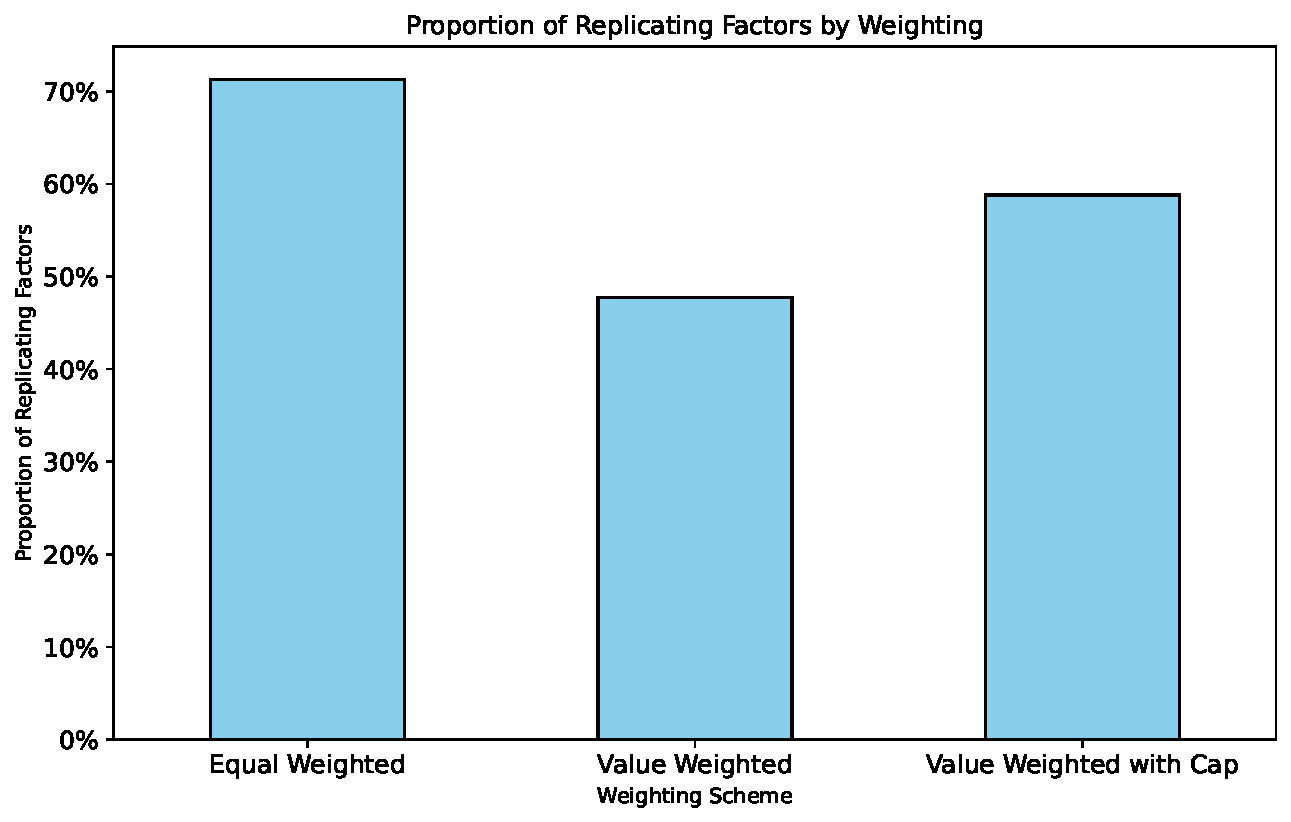
\includegraphics[width=.95\textwidth]{out/1.pdf}
\end{figure}

\FloatBarrier

\section{}
\begin{figure}[htbp]
    \centering
    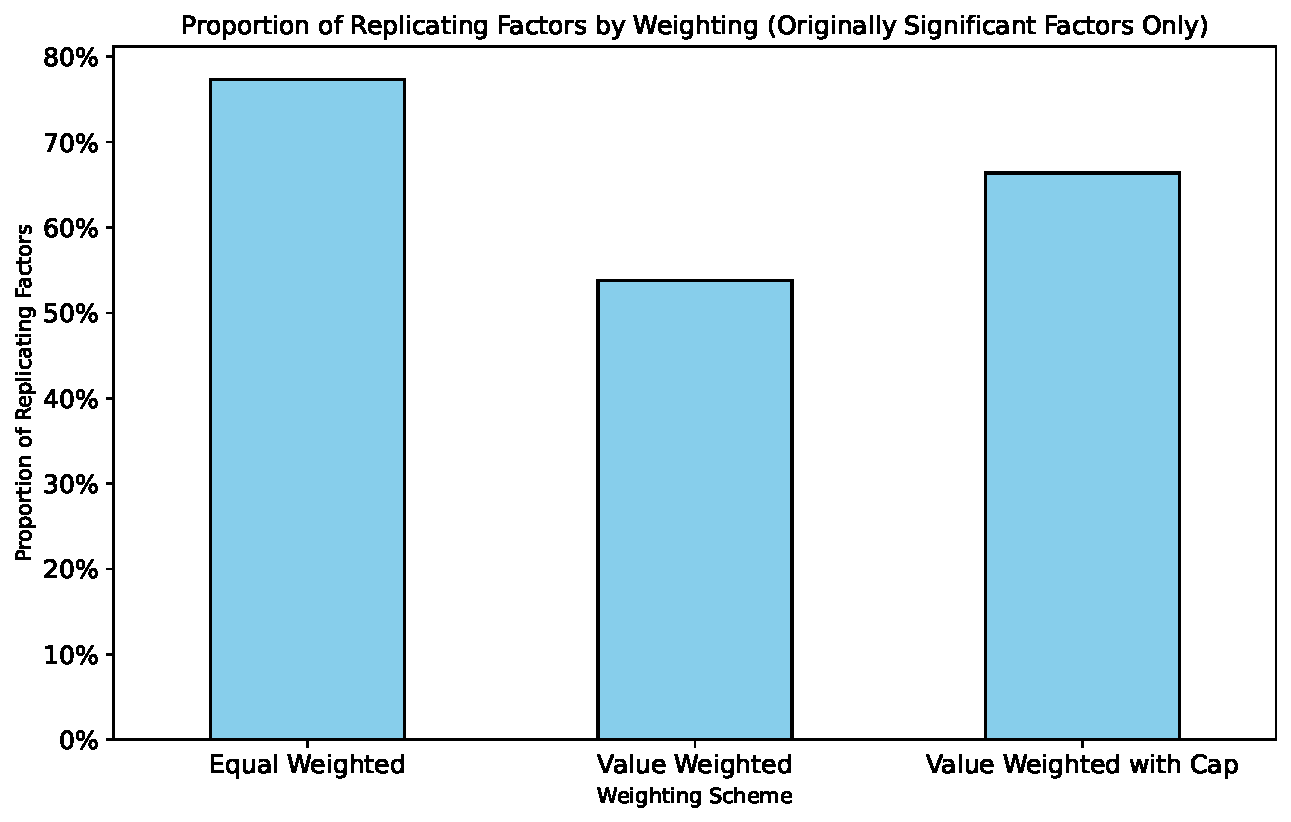
\includegraphics[width=.95\textwidth]{out/2.pdf}
\end{figure}

\FloatBarrier

\section{}
\begin{figure}[htbp]
    \centering
    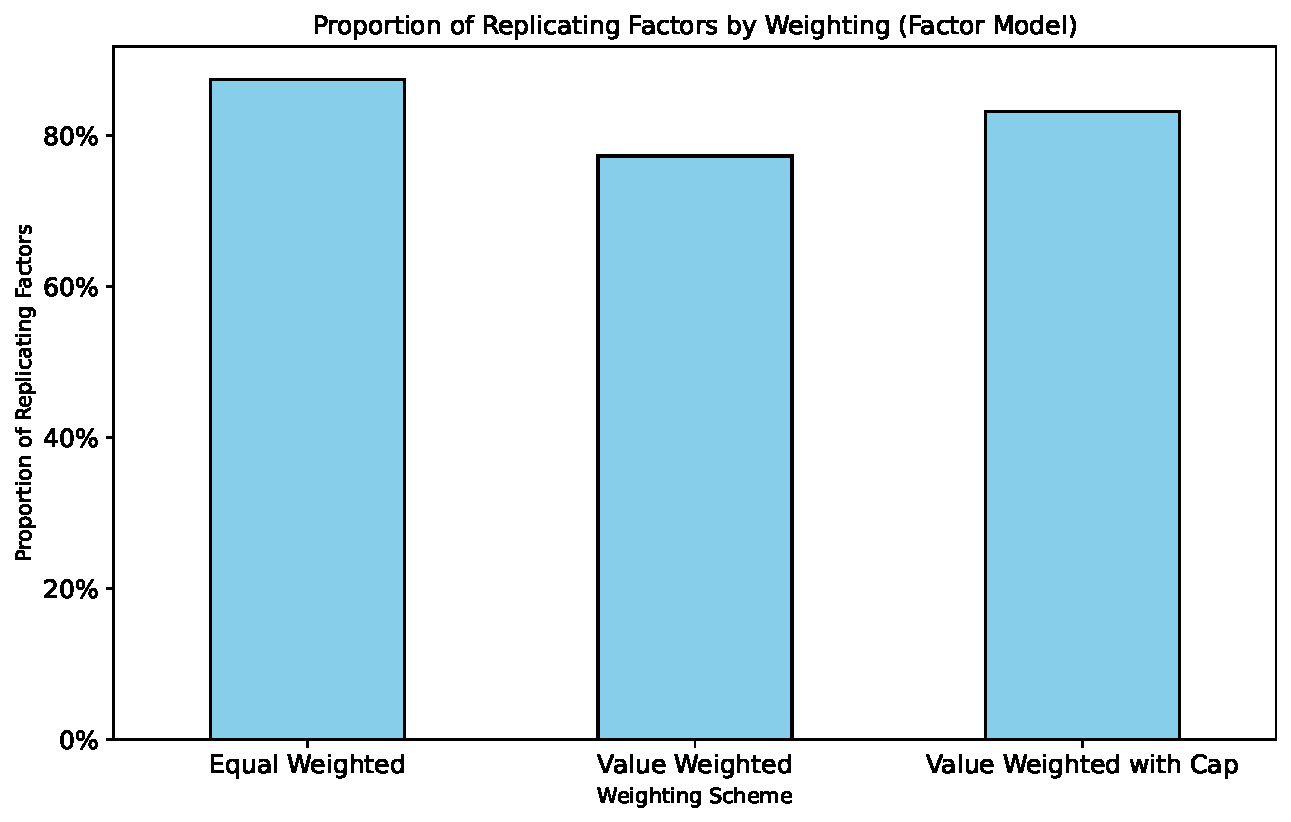
\includegraphics[width=.95\textwidth]{out/3.pdf}
\end{figure}

\FloatBarrier

\section{}
\begin{figure}[htbp]
    \centering
    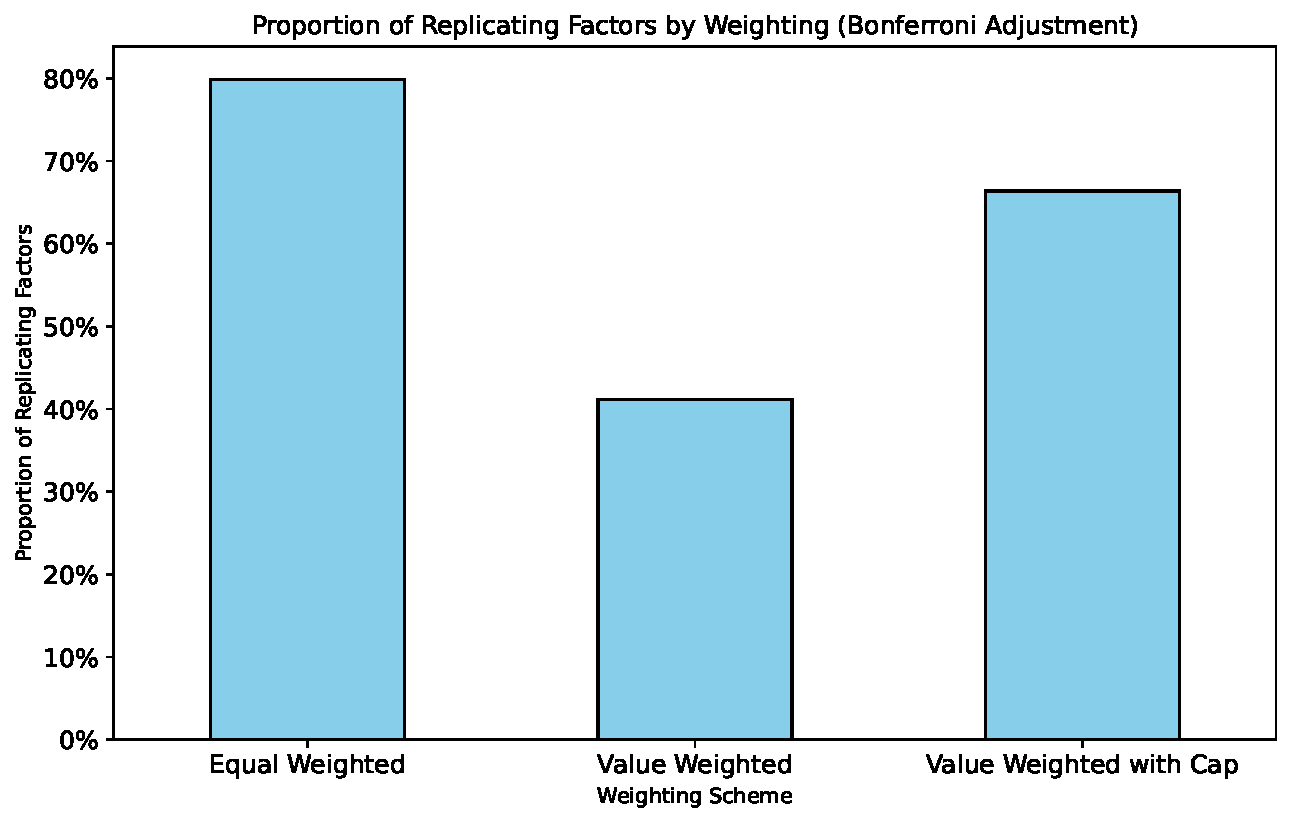
\includegraphics[width=.95\textwidth]{out/4.pdf}
\end{figure}

\FloatBarrier

\section{}
\begin{figure}[htbp]
    \centering
    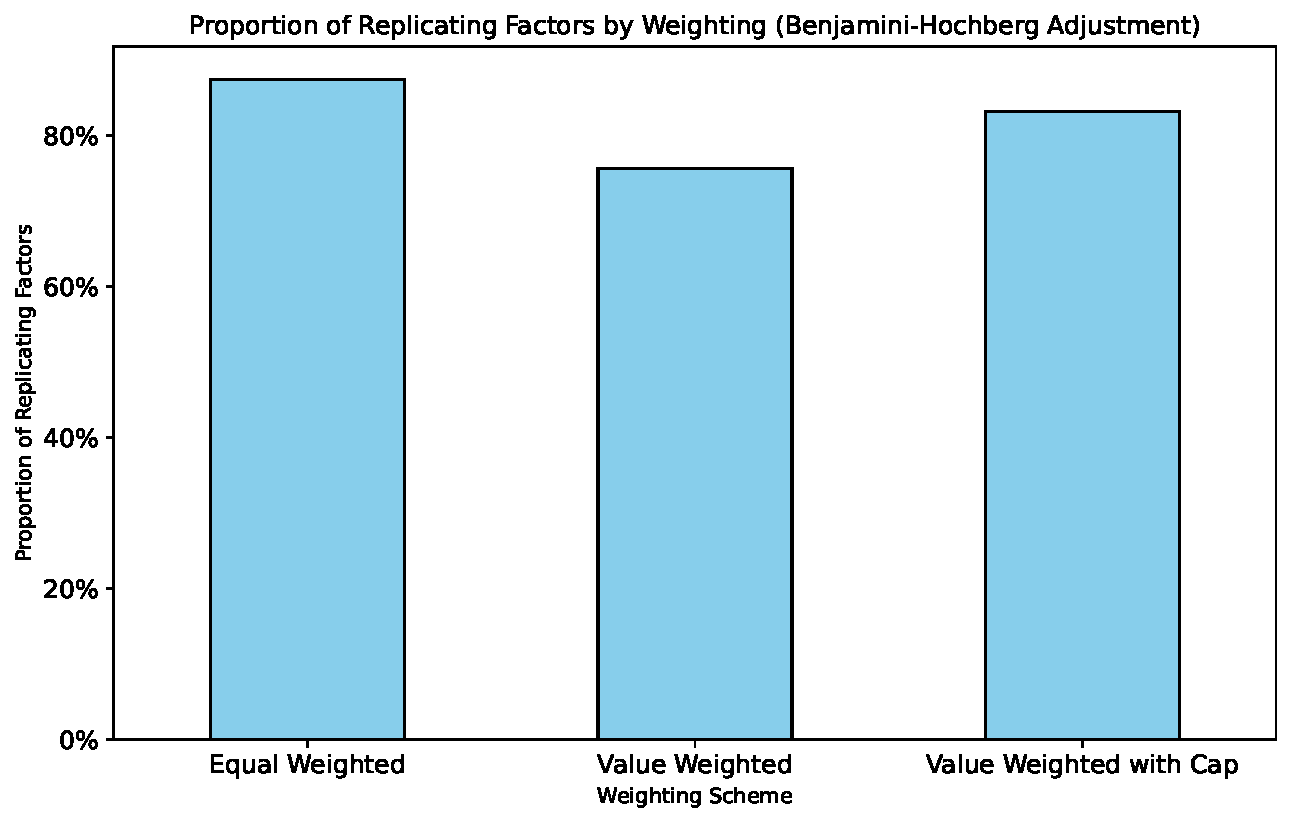
\includegraphics[width=.95\textwidth]{out/5.pdf}
\end{figure}

\FloatBarrier
\section{}
\begin{table}[htbp]
    \centering
    \resizebox{\textwidth}{!}{%
        \begin{tabular}{lccccccccccccc}
\toprule
{} &  Low Leverage &  Size &  Investment &  Value &  Low Risk &  Debt Issuance &  Quality &  Seasonality &  Accruals &  Profitability &  Profit Growth &  Short-Term Reversal &  Momentum \\
\midrule
Low Leverage        &          0.39 &  0.07 &       -0.29 &  -0.37 &     -0.34 &           0.06 &     0.07 &        -0.04 &     -0.01 &          -0.24 &           0.12 &                -0.12 &      0.04 \\
Size                &          0.07 &  0.33 &        0.05 &   0.01 &     -0.11 &           0.04 &    -0.09 &         0.02 &      0.02 &          -0.17 &          -0.09 &                -0.01 &     -0.12 \\
Investment          &         -0.29 &  0.05 &        0.39 &   0.32 &      0.24 &           0.09 &    -0.13 &         0.04 &      0.09 &           0.08 &          -0.14 &                 0.07 &     -0.02 \\
Value               &         -0.37 &  0.01 &        0.32 &   0.42 &      0.32 &          -0.02 &    -0.06 &         0.04 &      0.02 &           0.22 &          -0.15 &                 0.13 &     -0.11 \\
Low Risk            &         -0.34 & -0.11 &        0.24 &   0.32 &      0.40 &          -0.05 &     0.01 &         0.03 &     -0.03 &           0.26 &          -0.08 &                 0.14 &      0.01 \\
Debt Issuance       &          0.06 &  0.04 &        0.09 &  -0.02 &     -0.05 &           0.28 &     0.05 &         0.03 &      0.03 &          -0.03 &           0.08 &                -0.03 &      0.09 \\
Quality             &          0.07 & -0.09 &       -0.13 &  -0.06 &      0.01 &           0.05 &     0.29 &         0.02 &     -0.10 &           0.17 &           0.11 &                 0.02 &      0.08 \\
Seasonality         &         -0.04 &  0.02 &        0.04 &   0.04 &      0.03 &           0.03 &     0.02 &         0.07 &      0.01 &           0.03 &           0.01 &                 0.01 &      0.02 \\
Accruals            &         -0.01 &  0.02 &        0.09 &   0.02 &     -0.03 &           0.03 &    -0.10 &         0.01 &      0.27 &          -0.10 &          -0.01 &                -0.02 &     -0.01 \\
Profitability       &         -0.24 & -0.17 &        0.08 &   0.22 &      0.26 &          -0.03 &     0.17 &         0.03 &     -0.10 &           0.37 &           0.02 &                 0.11 &      0.01 \\
Profit Growth       &          0.12 & -0.09 &       -0.14 &  -0.15 &     -0.08 &           0.08 &     0.11 &         0.01 &     -0.01 &           0.02 &           0.24 &                -0.04 &      0.15 \\
Short-Term Reversal &         -0.12 & -0.01 &        0.07 &   0.13 &      0.14 &          -0.03 &     0.02 &         0.01 &     -0.02 &           0.11 &          -0.04 &                 0.28 &     -0.06 \\
Momentum            &          0.04 & -0.12 &       -0.02 &  -0.11 &      0.01 &           0.09 &     0.08 &         0.02 &     -0.01 &           0.01 &           0.15 &                -0.06 &      0.37 \\
\bottomrule
\end{tabular}

    }
\end{table}

\FloatBarrier

I calculate the $\Sigma^{\text{block}}$ and $C^{\text{block}}$ as mentioned in the exercise. 

\section{}
I could not manage to run the maximum likelihood estimation for estimating the $\tau_c$ and $\tau_w$ parameters. 

\appendix

\section*{Appendix}

Here you can find the python code that I used to solve the exercise. \href{https://github.com/mortezaaghajanzadeh/BDAP/tree/main/Assignments/Assignment3}{Link to the GitHub repository.}

\end{document}